%\color{red}
%objetivos de este capítulo
%\color{black}

En este capítulo estudiaremos un candidato a materia oscura tipo WIMP en el $\nu_R-331$, calcularemos su densidad de reliquia al resolver su ecuación de Boltzmann y compararemos el resultado con los valores del modelo cosmológico estándar $\Lambda$CDM.

\section[\hspace{-0.14in}Introduction]{Introducción} 
% ----------------------------------------------------------------------------------- 

Como vimos en el capítulo anterior, el campo $\eta_3^0$
\begin{equation}
\eta = \begin{pmatrix} \eta_1^0  \\ \eta_2^- \\  \eta_3^0 \end{pmatrix}
\end{equation}
solo acopla con quarks ligeros a través del acople con los quarks pesados\footnote{Asumiendo que el tercer miembro de cada triplete (o antitriplete) de fermiones es un autoestado de masa \cite{Buras:2012dp,Cao:2016uur}. También se puede usar una simetria $\mathbb{Z}_2$ que prohiba la mezcla entre quarks del ME y los nuevos $u_4,d_4$ y $d_5$ \cite{Okada:2016whh}.} $u_4,d_4$ y $d_5$,
\begin{equation}
\text{Q}_{1L} = \left( \begin{array}{c}
u_1 \\ d_1  \\ u_4
\end{array} \right)_{L},  
\text{Q}_{2L} = \left( \begin{array}{c}
d_2 \\ u_2  \\ d_{4}
\end{array} \right)_L, 
\text{Q}_{3L} = \left( \begin{array}{c}
d_3 \\ u_3  \\ d_{5}
\end{array} \right)_L, 
\end{equation}
via el siguiente lagrangiano de Yukawa
\begin{equation}
-\mathcal{L}^{\eta_3^0}_{\rm Yuk} = \beta_a \bar{u}_{4L} u_{aR}\eta_3^0 + \beta_{2a} \bar{d}_{4L} d_{aR}\eta_3^0 + \beta_{3a} \bar{d}_{5L} d_{aR}\eta_3^0 \hspace{0.1in} (a=1,2,3).
\end{equation}
Los escalares físicos
\begin{equation}
\eta_R = \frac{v_\eta}{v_\chi} \text{Re}(\chi_1^0) + \text{Re}(\eta_3^0) \hspace{0.3in} y \hspace{0.3in} \eta_I = -\frac{v_\eta}{v_\chi} \text{Im}(\chi_1^0) + \text{Im}(\eta_3^0)
\end{equation}
se aproximan a la parte real e imaginaria de $\eta_3^0$ ya que $v_\chi \gg v_\eta$ por ser la mayor escala de energía del modelo,
\begin{equation}
\eta_R \approx \text{Re}(\eta_3^0), \hspace{0.3in} \eta_I \approx \text{Im}(\eta_3^0).
\end{equation}
Sin embargo, sus masas aún permanecen diferentes
\begin{equation}
m_{\eta_R}^2 \approx \frac{1}{2} \bigg( \lambda_8 +2\lambda_{10}  \bigg) v_\chi^2 \hspace{0.3in} y \hspace{0.3in} m_{\eta_I}^2 \approx \frac{1}{2} \bigg( \lambda_8 -2\lambda_{10}  \bigg) v_\chi^2,
\end{equation}
por lo que a partir de ahora trabajaremos en el límite de $\lambda_{10} \to 0$, ya que en ese caso el candidato a materia oscura será el escalar complejo $\eta_3^0$, 
\begin{equation}
\mathcal{DM} \equiv \eta_3^0 =  {\rm Re}(\eta_3^0) + i \, {\rm Im}(\eta_3^0)
\end{equation}
con masa
\begin{equation}
m_\mathcal{DM}=m_{\eta_R}=m_{\eta_I} = \sqrt{\frac{\lambda_8}{2} } \, v_\chi.
\end{equation}



%Un buen candidato a materia oscura necesita ser estable o, en su defecto, tener un tiempo de vida media mucho más grande que la edad actual del universo $13.8$ Gyr \cite{Workman:2022ynf}. Debido a los vértices $HAZ$, $HH^{\pm}W^{\mp}$ y $AH^{\pm}W^{\mp}$, tanto $H$ como $A$ pueden decaer, siempre que el proceso sea cinemáticamente permitido. Del cuadro \ref{masses331} vemos que los escalares cargados son más pesados que $A$, lo que nos induce a pensar que si $m_H < m_A$, entonces $H$ podría ser estable o de larga vida. Esto se debe a que aún podría decaer en quarks y leptones. A continuación vamos a demostrar que en nuestro caso de interés ($f\, v_\chi = v_{\rm SM}^2$) existe una región amplia del espacio de parámetros donde se cumple esta desigualdad.



% -------------------------------------------------------------------------------------
\section[\hspace{-0.14in}Sección de choque térmica]{Sección de choque térmica}
% -------------------------------------------------------------------------------------

El promédio térmico de la sección de choque de aniquilación multiplicada por la rapidéz relativa de las partículas de materia oscura\footnote{A partir de ahora la llamaremos de forma abreviada como sección de choque térmica.} $\left< \sigma v \right>$ es una cantidad muy importante para la fenomenología. Esta es parte fundamental de la ecuación de Boltzmann para calcular la densidad de reliquia de la materia oscura, $\Omega_{\mathcal{DM}}$ (ver apéndice),
\begin{equation}
\dot{n} + 3Hn = \langle \sigma v \rangle \left( n_{\rm eq}^2 - n^2 \right).
\end{equation}
Resolviendo esta ecuación obtenemos la densidad numérica de las partículas de materia oscura $n$ y con ello
\begin{equation}
\Omega_{\mathcal{DM}} = \frac{\rho}{\rho_c} = \frac{m_{\mathcal{DM}}}{\rho_c} \left(n_{\eta_R}+n_{\eta_I}\right).
\end{equation}
Para gases no relativistas, una buena aproximación para obtener la sección de choque térmica se obtiene al expandir la sección de choque en potencias de $x^{-1} \equiv T/m_{\mathcal{DM}}$. Esto se logra aproximando la energía del centro de masa $\sqrt{s}$ como
\begin{equation}
s \approx 4m_\mathcal{DM}^2+m_\mathcal{DM}^2 v_{\text{rel}}^2,
\end{equation}
donde $v_\text{rel}=2v$ es la `velocidad' relativa entre las partículas de materia oscura,
\begin{equation}
E_K = \frac{3}{2}k_BT = \frac{1}{2}m_\mathcal{DM} v^2,
\end{equation}
 y $k_B$ es la constante de Boltzmann.

La forma exacta de la sección de choque térmica fue publicada en la referencia \cite{gondolo1991cosmic} y esta se muestra en la ecuación \ref{svMol}.

%y posteriormente se encontraron excepciones importantes al cálculo de estas abundancias \cite{Griest:1990kh}. Por ejemplo, la aniquilación de materia oscura en partículas más pesadas está prohibida cinemáticamente, sin embargo, si esta diferencia de masas no es muy grande, este canal puede ser dominante y determinar la densidad de la materia oscura.

%Para la detección indirecta de materia oscura, que es lo que nos interesa en este trabajo, calculamos $\left< \sigma v \right>$ en el límite que $v\to 0$. En este caso, basta calcular la sección de choque de aniquilación $\sigma$ y multiplicarla por la rapidéz relativa $v$ de las partículas de materia oscura, las cuales hemnos asumido que son no relativisticas.


\subsection[\hspace{-0.4in}) Diagramas de Feynman]{Diagramas de Feynman}
En el $\nu_R-331$ que hemos descrito, nuestro candidato a materia oscura podría aniquilarse a nivel de árbol a través de los procesos mostrados en la figura \ref{Feynman_diagrams},
\begin{figure}[h]
\centering
\begin{minipage}{.35\textwidth}
  \centering
  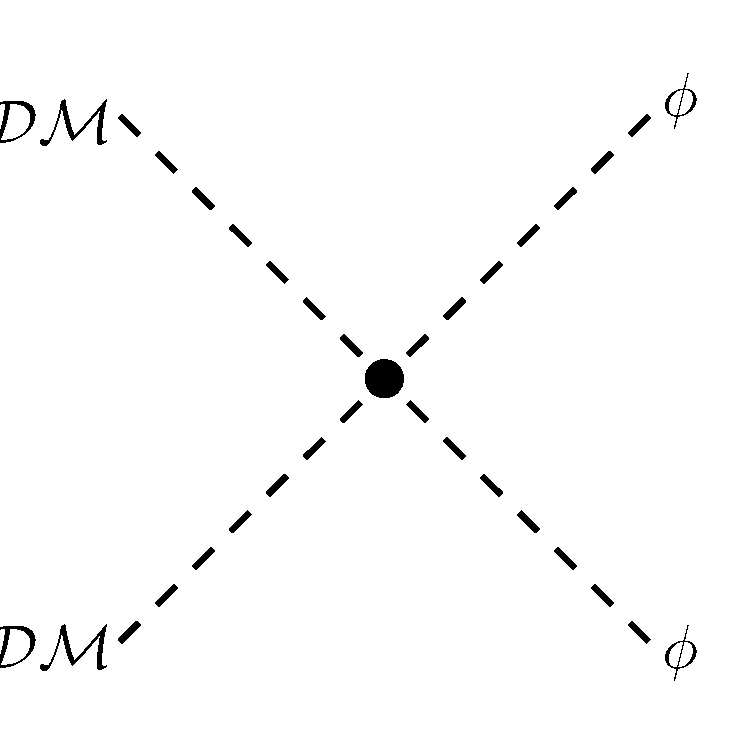
\includegraphics[height=1.2in]{Images/DM_ann_1.pdf}
  \caption*{(a)}
%  \label{fig:test1}
\end{minipage}%
\centering
\begin{minipage}{.35\textwidth}
  \centering
  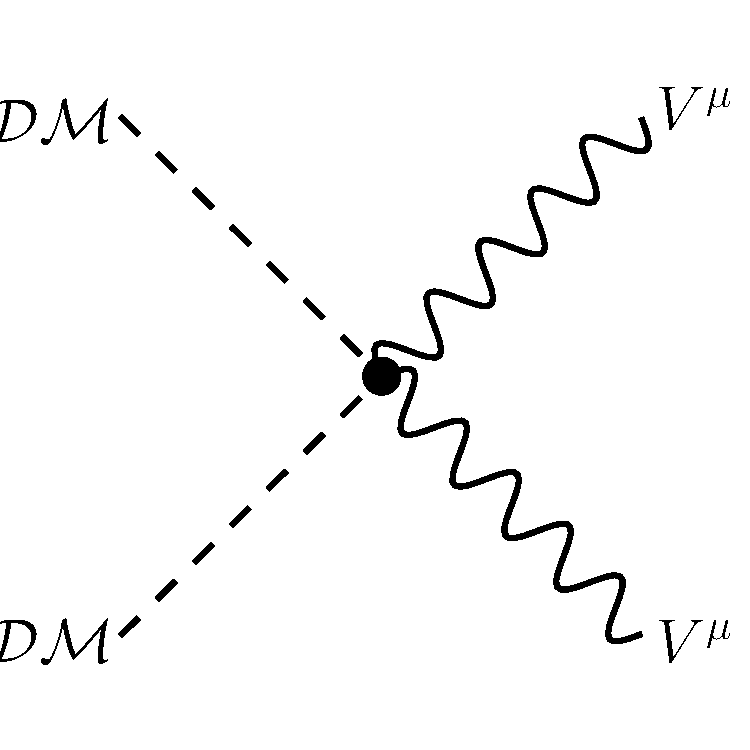
\includegraphics[height=1.2in]{Images/DM_ann_2.pdf}
  \caption*{(b)}
%  \captionof{figure}{A figure}
%  \label{fig:test1}
\end{minipage}% 
\centering
\begin{minipage}{.35\textwidth}
  \centering
  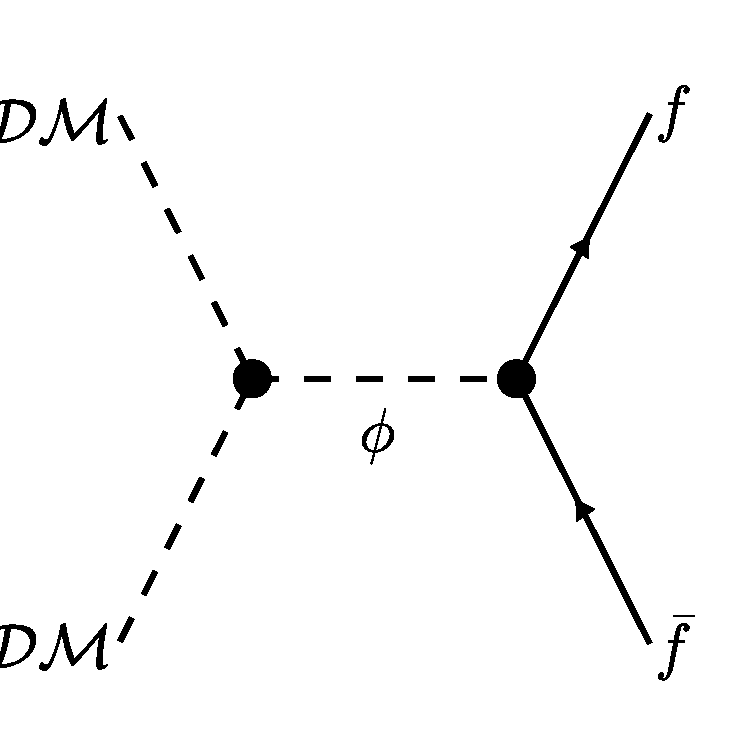
\includegraphics[height=1.2in]{Images/DM_ann_3.pdf}
  \caption*{(c)}
%  \captionof{figure}{A figure}
%  \label{fig:test1}
\end{minipage}% 
\vspace{0.25in}
\centering
\begin{minipage}{.35\textwidth}
  \centering
  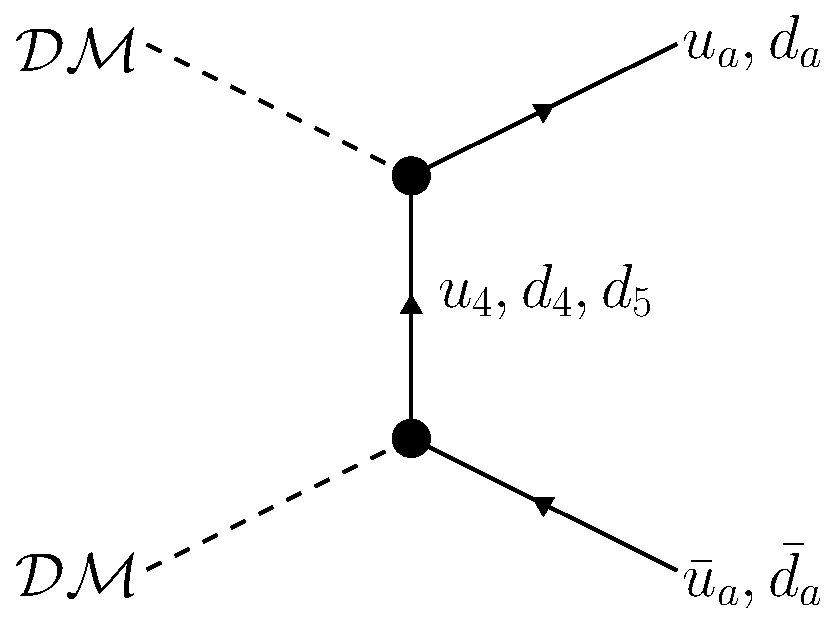
\includegraphics[height=1.2in]{Images/DM_ann_4.pdf}
  \caption*{(d)}
%  \captionof{figure}{A figure}
%  \label{fig:test1}
\end{minipage}% 
\begin{minipage}{.35\textwidth}
  \centering
  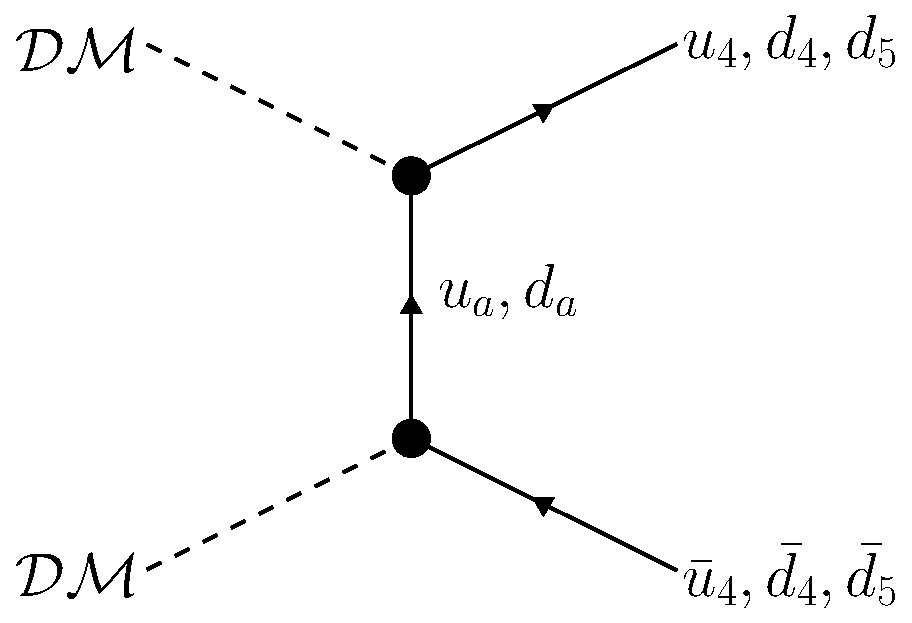
\includegraphics[height=1.2in]{Images/DM_ann_6.pdf}
  \caption*{(f)}
%  \captionof{figure}{A figure}
%  \label{fig:test1}
\end{minipage}% 
\caption[\hspace{0.05in}Aniquilación de materia oscura en el $\nu_R-$331]{Aniquilación de materia oscura: procesos que cambian el numero de partículas de materia oscura a nivel de árbol. En (a) tenemos $\phi=h,H,H_3, A,H^{\pm},\eta^{\pm}$, en (b) $V^{\mu} = Z^{\mu},Z'^{\mu},Y_1^{\mu},Y_2^{\mu},W'^{\mu}$, en (c) $\phi = h,H,H_3$ y en (d) tenemos $u_a=u,c,t$ y $d_a=d,s,b$.} 
\label{Feynman_diagrams}
\end{figure}
y también podría decaer en quarks por medio del vértice mostrado en la figura \ref{fig:DMdecay}.
\begin{figure}[h]
\centering
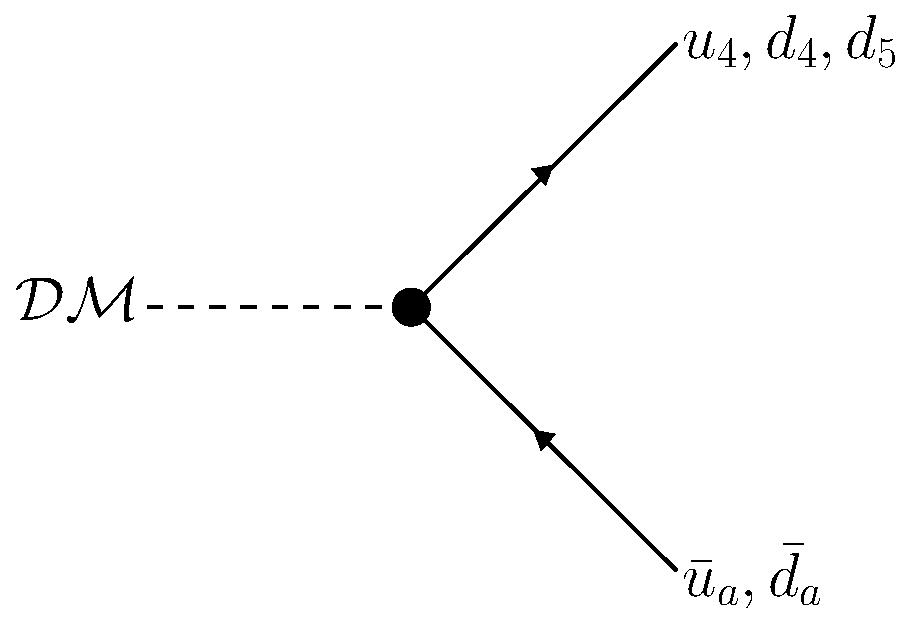
\includegraphics[scale=0.35]{Images/DM_decay.pdf}
\caption[\hspace{0.05in}Posible canal de decaimiento de la materia oscura]{Diagrama de Feynman que podría inducir al decaimiento del candidato a materia oscura en quarks.}
\label{fig:DMdecay}
\end{figure}
Debido a que estamos buscando un candidato a materia oscura, este deberia ser estable o tener un tiempo de vida media mucho mayor a la edad del universo. Tomaremos la primera opción al hacer que estos decaimientos sean cinemáticamente prohibidos, $m_\mathcal{DM} < m_{Q} + m_q$, donde $Q=u_4,d_4,d_5$ y $q=u,d,c,s,t,b$, ya que en el otro caso deberíamos hacer muchos ajustes finos.

\newpage

\subsection[\hspace{-0.4in}) Sección de choque térmica $\langle \sigma v \rangle$]{Sección de choque térmica $\langle \sigma v \rangle$}

Generalmente el candidato a materia oscura es la partícula más ligera del sector oscuro y por este motivo trabajaremos con la siguiente jerarquia: $m_\mathcal{DM} < m_{H_3},m_{\eta^\pm},m_{Y_1},m_{Y_2},m_{Z'},m_{W'}$. Esto restringe varios de los procesos mostrados en la figura \ref{Feynman_diagrams}.

A continuación mostramos las secciones de choque térmicas aproximadas para los diagramas de la figura \ref{Feynman_diagrams} que consideramos cinemáticamente permitidos.

%\newpage

\begin{equation}
\langle \sigma_{\mathcal{DM} \ \mathcal{DM} \to \phi \phi} \, v \rangle \approx \frac{g_4^2}{32\pi m_\mathcal{DM}^2} \left(1-\left( \frac{m_\phi}{m_\mathcal{DM}}\right)^2 \right)^{1/2}
\end{equation}


\begin{equation}
\langle \sigma_{\mathcal{DM} \ \mathcal{DM} \to f \bar{f}} \, v \rangle \approx \frac{g_\phi^2 g_f^2}{32\pi (m_\phi^2-4m_\mathcal{DM}^2)^2} \left( 1- \left( \frac{m_f}{m_\mathcal{DM}} \right)^2 \right)^{3/2}
\end{equation}


\begin{equation}
\langle \sigma_{\mathcal{DM} \ \mathcal{DM} \to q \bar{q}} \, v \rangle \approx \frac{g_q^4\left(m_Q+m_q\right)^2 }{16\pi (m_Q^2-m_q^2+m_\mathcal{DM}^2)^2 } \left( 1-\left(\frac{m_q}{m_\mathcal{DM}} \right)^2 \right)^{3/2}  
\end{equation}

donde $g_4,g_\phi,g_f$ y $g_q$ son el acople cuartico, con escalares, con fermiones y con quarks, respectivamente.

\begin{figure}[h]
\centering
\begin{minipage}{.5\textwidth}
  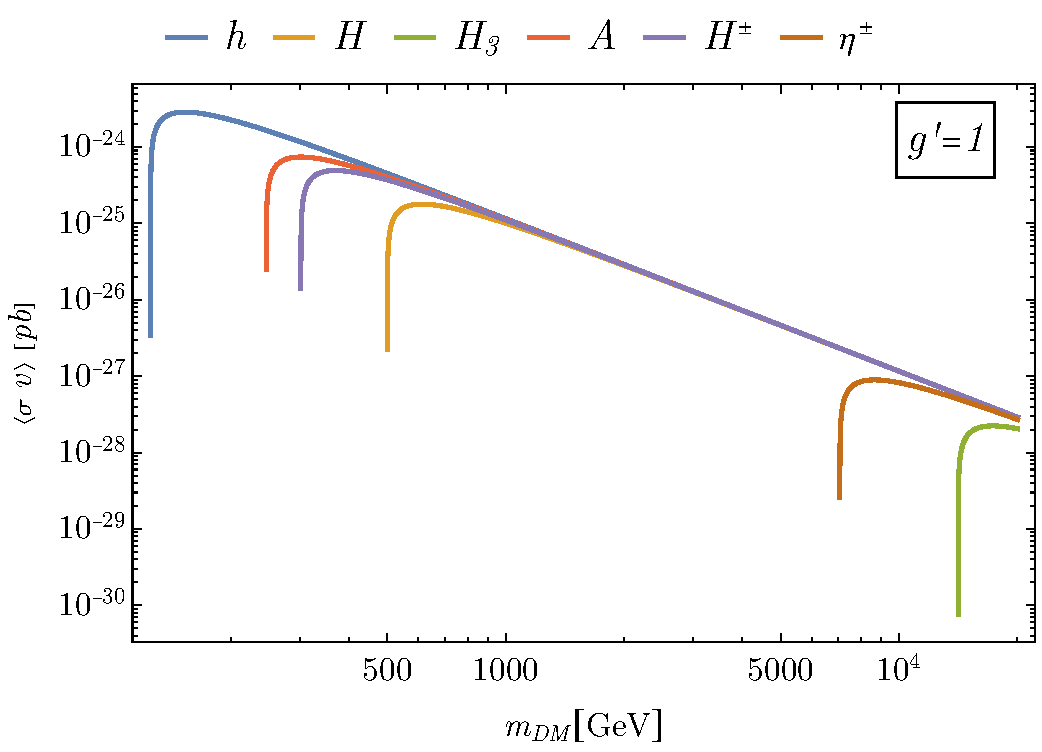
\includegraphics[height=1.88in]{Results/sv-a.pdf}
\end{minipage}%
\centering
\begin{minipage}{.5\textwidth}
  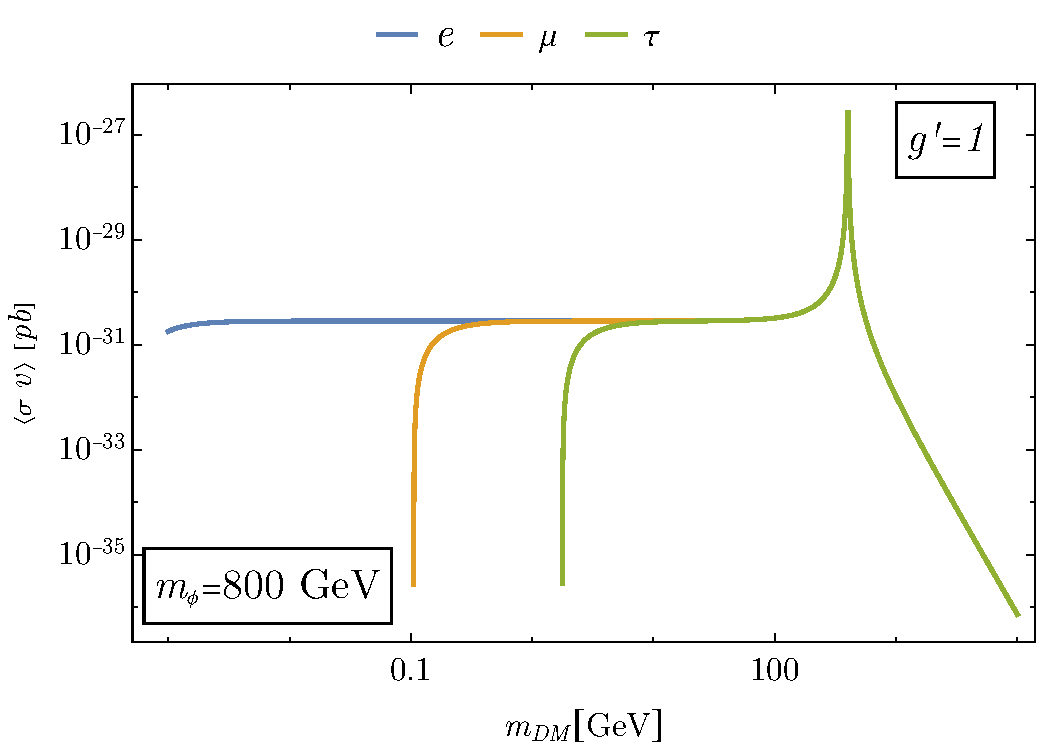
\includegraphics[height=1.88in]{Results/sv-c.pdf}
\end{minipage}% 
\ \
\centering
\begin{minipage}{\textwidth}
  \centering
  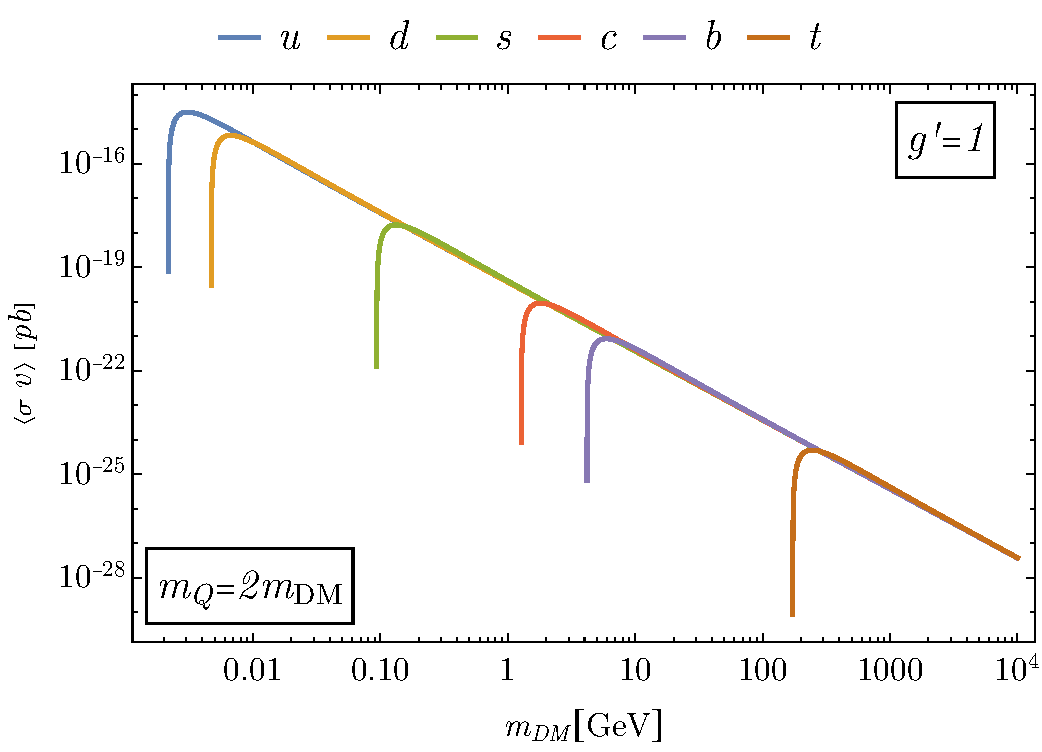
\includegraphics[height=1.88in]{Results/sv-d.pdf}
\end{minipage}% 
\caption[\hspace{0.1in}Sección de choque térmica $\langle \sigma v \rangle$]{Sección de choque térmica $\langle \sigma v \rangle$ para los diagramas de Feynman (a), (c) y (d) de la figura \ref{Feynman_diagrams}. \textbf{(Izquierda)} Las masas de los escalares están de acuerdo con la restricción de que la masa del Higgs debe estar en $m_h = 125.20 \pm 0.11$ GeV. \textbf{(Derecha)} Consideramos solo leptones y fijamos la masa del escalar intermediario $m_H=$800 GeV. \textbf{(Abajo)} Fijamos la masa del quark pesado intermediario como el doble de la masa de la materia oscura $m_Q = 2m_\mathcal{DM}$. Cuando la masa de la materia oscura es más pesada que la del quark top, todas las secciones de choque térmicas son del mismo valor. } 
\label{sv}
\end{figure}

\newpage

\section[\hspace{-0.14in}Densidad de relíquia]{Densidad de relíquia}
Para calcular la densidad actual de materia oscura $\Omega_{\mathcal{DM}}$ debemos resolver la ecuación de Boltzmann,
\begin{equation}
\frac{d\Upsilon}{dx} = -\frac{x\left< \sigma v \right>s}{H(m)} \left( \Upsilon^2 - \Upsilon^2_{\rm eq} \right),
\end{equation}
donde $m$: masa de la materia oscura, $T$: temperatura del plasma primordial, $x\equiv m/T$, $n$: densidad numérica de materia oscura, $s$: densidad de entropía, 
\begin{equation}
s = \frac{2\pi^2}{45} g_{*S}(T) T^3,
\end{equation}
$g_{*S}(T)$ son los grados de libertad de entropía (ver figura \ref{reldof}), $\Upsilon \equiv n/s$, $H$: parámetro de Hubble-Lema\^itre en la época de radiación (ver apéndice),
\begin{equation}
H = \frac{1.66}{M_{\rm Pl}} \sqrt{g_*(T)}T^2,
\end{equation}
$g_*(T)$ son los grados de libertad relativistas, $M_{\rm Pl}=1/\sqrt{G_N}$ , $H(m)=x^2 H(T)$, $\Upsilon_{\rm eq}$: la función de equilibrio para especies no relativistas \cite{gondolo1991cosmic}, 
\begin{equation}
\Upsilon_{\rm eq}(x) = \frac{45}{2\pi^4} (2s+1) \frac{x^2}{g_{*S}(T)}K_{2}(x),
\end{equation}
donde $s:$spin de la materia oscura, $K_{2}(x)$: función de Bessel modificada de segundo tipo, $\left< \sigma v \right>$: sección de choque de aniquilación térmica total \cite{Kolb:1990vq},
\begin{equation}
\sigma = \sum_X \sigma(\mathcal{DM} \, \overline{\mathcal{DM}} \to X \bar{X}),
\end{equation}
donde se asume que todas las espécies $X$ tienen distribuciones térmicas y potencial químico nulo. 

Para calcular $\left< \sigma v \right>$ usamos \cite{gondolo1991cosmic},
\begin{equation}
\left< \sigma v_{\rm Mol} \right> = \frac{1}{8m^4TK_2^2(m/T)} \int_{4m^2}^\infty \sigma (s-4m^2)\sqrt{s}K_1(\sqrt{s}/T)ds,
\label{svMol}
\end{equation}
donde $v_{\rm Mol}=(|\vec{v}_1-\vec{v}_2|^2-|\vec{v}_1 \times \vec{v}_2|^2)^{1/2}.$ Con esto obtenemos $\rho_{\mathcal{DM}} = m_\mathcal{DM} \, n$ y finalmente $\Omega_{\mathcal{DM}}= \rho_\mathcal{DM}/\rho_{c,0}$.

Las observaciones cosmológicas indican que la materia oscura debe ser (en su mayoria) fria. Esto quiere decir que la cantidad $x=m_\mathcal{DM}/T$, donde $m_\mathcal{DM}$ es la masa de la materia oscura y $T$ es la temperatura del plasma primordial, debe ser mayor que la unidad al momento del freeze-out. Generalmente $x_{f.o}\sim \mathcal{O}(10)$ para WIMPs \cite{profumo2017introduction}. Por ejemplo, para un materia oscura de $m_\mathcal{DM}=1$ TeV y $x_{f.o}=20$, tenemos
\begin{equation}
x_{f.o}=\frac{m_\mathcal{DM}}{T} = \frac{1 \text{ TeV}}{T}=20 \Longrightarrow T = 50 \text{ GeV}
\end{equation}
al momento del freeze-out. A esta temperatura, las partículas del modelo estándar son relativistas con excepción de los bosones vectoriales masivos, el Higgs y el quark top.

\begin{figure}[h]
\centering
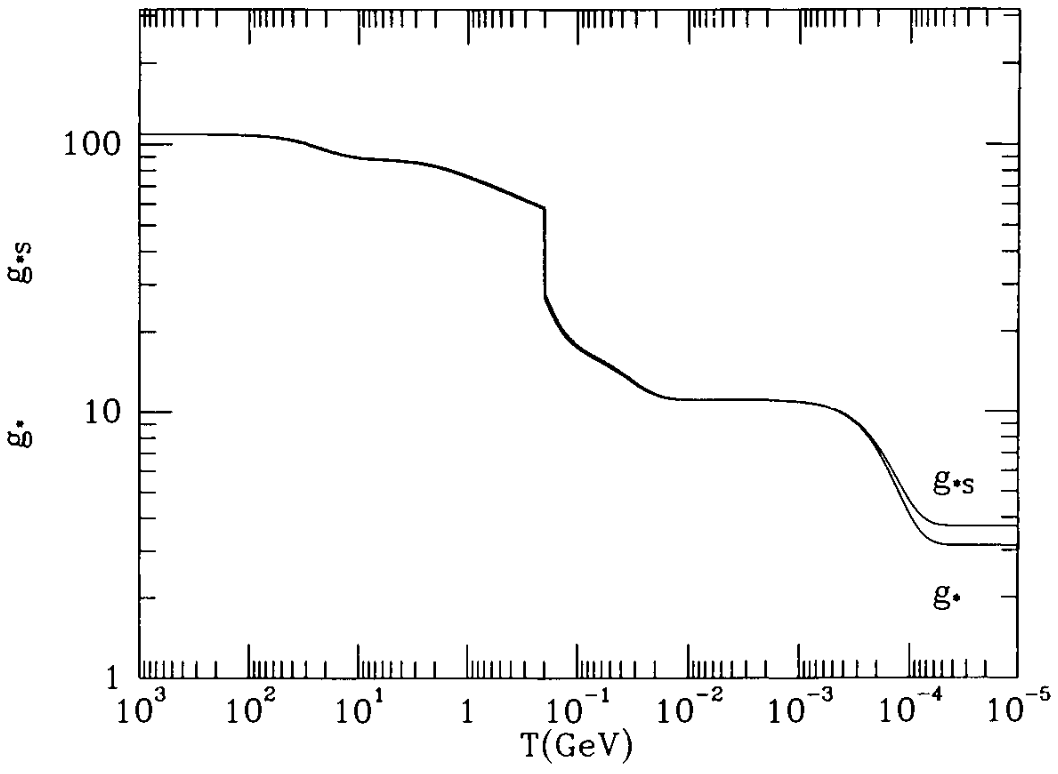
\includegraphics[scale=0.3]{Images/gstar.png}
\caption[\hspace{0.1in}Grados de libertad relativistas y de entropía]{Grados de libertad relativistas $g_*$ y grados de libertad de entropía $g_{*S}$ \cite{Kolb:1990vq}.}
\label{reldof}
\end{figure}


\newpage
\subsection[\hspace{-0.4in}) Resultados]{Resultados}

Debido a que existen varios tipos de procesos que pueden determinar la abundancia de la materia oscura en este modelo y, además, los estados finales son variados, decidimos simplificar el problema al elegir que solo uno de ellos sea dominate. 

Primeramente, elegimos el proceso mostrado en el diagrama (a) de la figura \ref{Feynman_diagrams} donde el proceso de aniquilación en escalares se da por un acople cuártico. En la figura \ref{Results-scalars} mostramos dos casos donde  conseguimos la abundancia correcta de materia oscura para $m_\mathcal{DM}$ cerca de 800(1200) GeV y $m_\phi=$ 0.9(0.1) $m_\mathcal{DM}$, cuando el acople es la unidad.

\begin{figure}[h]
\centering
\begin{minipage}{.5\textwidth}
  \centering
  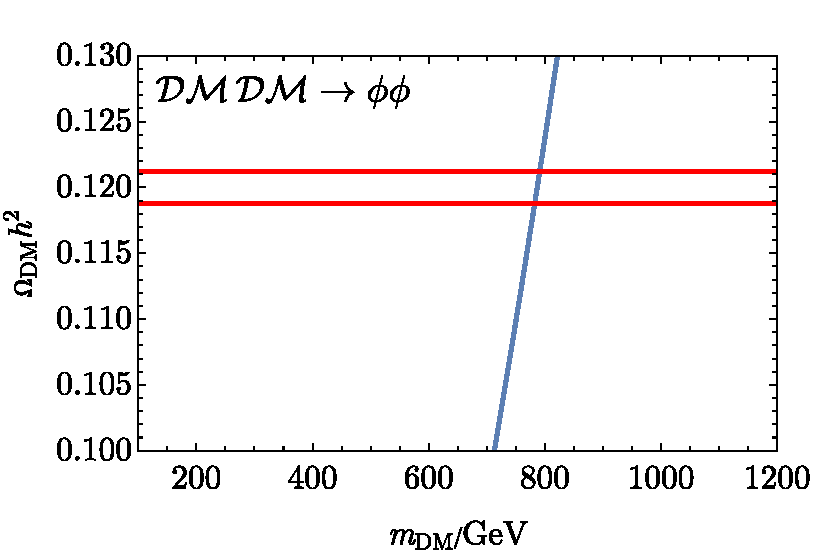
\includegraphics[height=2in]{Results/scalars-1.pdf}
%  \label{fig:test1}
\end{minipage}%
\centering
\begin{minipage}{.5\textwidth}
  \centering
  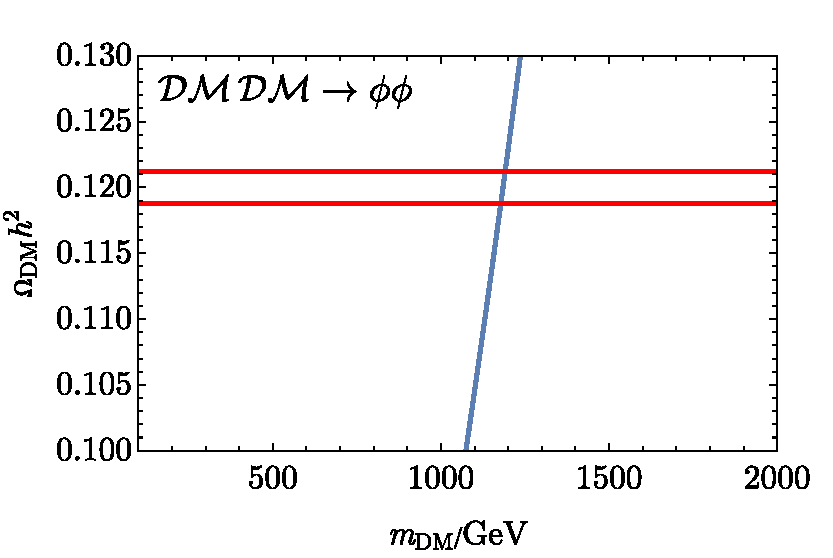
\includegraphics[height=2in]{Results/scalars-2.pdf}
%  \captionof{figure}{A figure}
%  \label{fig:test1}
\end{minipage}% 
\caption[\hspace{0.1in}Abundancia de materia oscura 1]{Abundancia de materia oscura dada por el proceso de la figura \ref{Feynman_diagrams} (a) cuando el acople cuartico entre los escalares $\phi$ y la materia oscura es $g'=1$ y los otros acoples de los demás diagramas son nulos. A la izquierda tenemos el caso $m_\phi =0.9\, m_\mathcal{DM}$ y a la derecha $m_\phi =0.1\, m_\mathcal{DM}$. Las lineas rojas delimitan la región de valores permitidos para $\Omega_{\mathcal{DM}}h^2$.} 
\label{Results-scalars}
\end{figure}


A continuación, mostramos los resultados para el diagrama (c) donde la materia oscura se aniquila en fermiones. Este proceso es mediado por un escalar $\phi$. Debido a que es el canal $s$, se espera una resonancia cuando $m_\mathcal{DM}=2 m_\phi$. Esto se muestra en la figura \ref{Results-fermions} asi como en la figura \ref{sv} para la sección de choque térmica. En este resultado, hemos trabajado con $m_\phi=$800 GeV y hemos ampliado la zona de interés (alrededor de $m_\phi/2 =400$ GeV) para mostrar las regiones donde reproducimos la correcta abundancia de materia oscura. Nótese que no mostramos los valores de las masas de los fermiones ya que estos influyen muy poco debido al factor $(m_f/m_\mathcal{DM})^2$.

\begin{figure}[h]
\centering
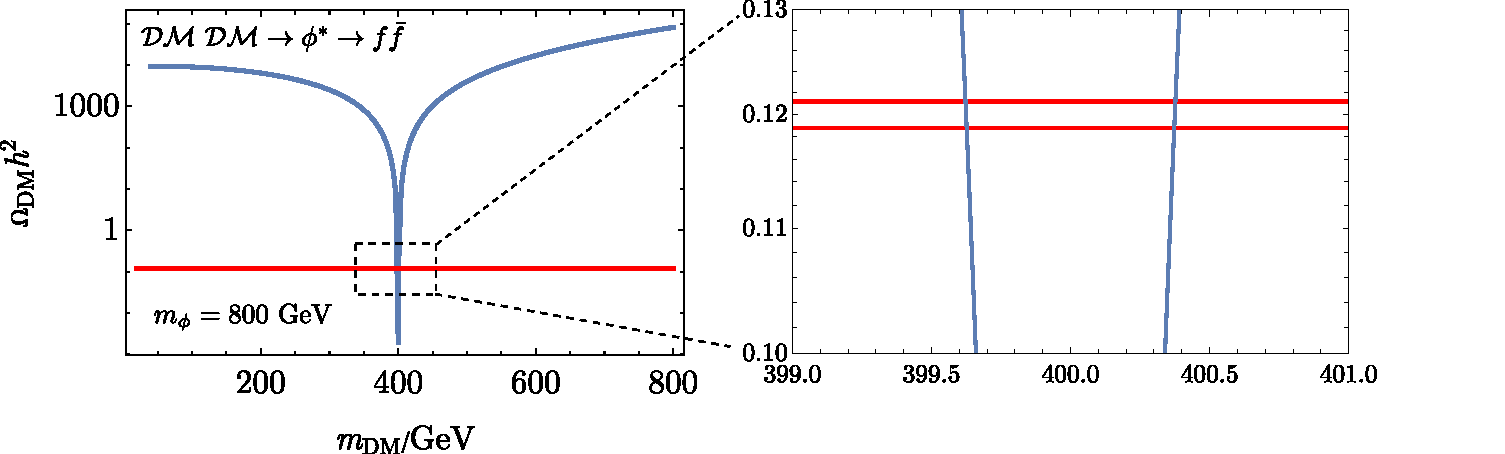
\includegraphics[scale=0.6]{Results/fermions.pdf}
\caption[\hspace{0.1in}Abundancia de materia oscura 2]{Abundancia de materia oscura dada por el proceso de la figura \ref{Feynman_diagrams} (c) cuando $m_\phi=800$ GeV y los acoples $\mathcal{DM}-\phi$ y $\phi-f$ son iguales a 1 (los otros son nulos). A la izquierda tenemos el scan completo en $m_\mathcal{DM}$ y a la derecha hacemos zoom a la región donde se cumplen los valores experimentales. Las lineas rojas delimitan la región de valores permitidos para $\Omega_{\mathcal{DM}}h^2$.}
\label{Results-fermions}
\end{figure}

%\vspace{1in}

Finalmente, trabajamos con el proceso dado por el del diagrama (d) de la figura \ref{Feynman_diagrams} el cual relaciona a la materia oscura con quarks del modelo estándar y los nuevos quarks super pesados $Q=u_4,d_4,d_5$ de los modelos $3-3-1$. En la referencia \cite{Okada:2016whh} se hace notar que debido a este acople, este candidato a materia oscura seria bueno ya que no acopla directamente con otros fermiones del modelo estándar, evitando limites experimentales actuales. Nuestros resultados se muestran en la figura \ref{Results-quarks} donde vemos que para masas $m_Q=2(10)m_\mathcal{DM}$ obtenemos la abundancia correcta cuando $m_\mathcal{DM}$ está alrededor de 480(125) GeV.


\begin{figure}[h!]
\centering
\begin{minipage}{.5\textwidth}
  \centering
  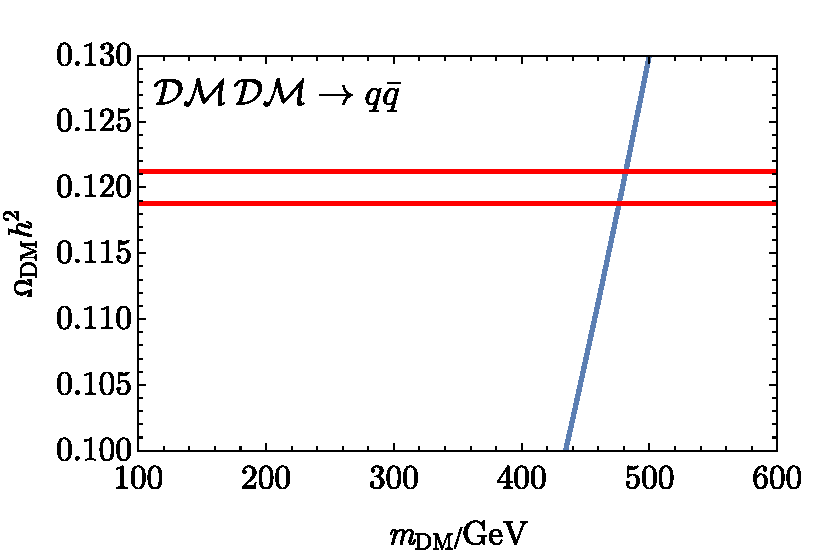
\includegraphics[height=2in]{Results/quarks-1.pdf}
%  \label{fig:test1}
\end{minipage}%
\centering
\begin{minipage}{.5\textwidth}
  \centering
  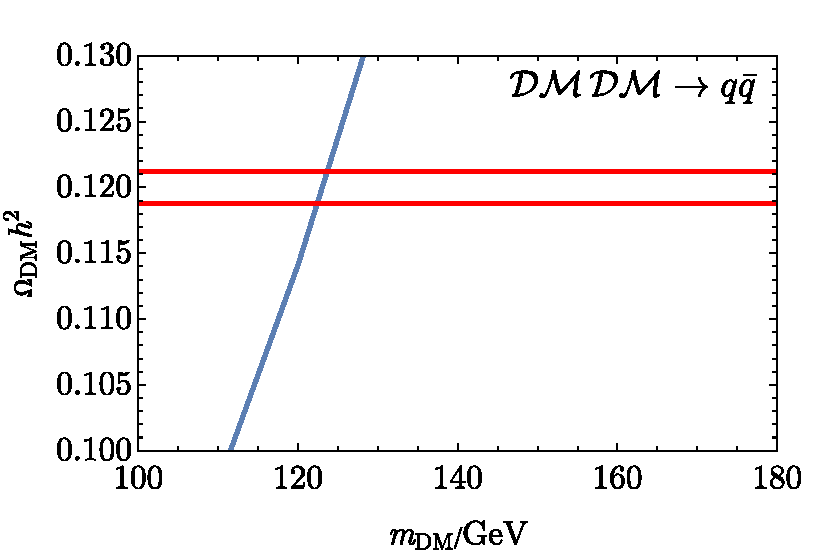
\includegraphics[height=2in]{Results/quarks-2.pdf}
%  \captionof{figure}{A figure}
%  \label{fig:test1}
\end{minipage}% 
\caption[\hspace{0.15in}Abundancia de materia oscura 3]{Abundancia de materia oscura via aniquilación por el canal $t$ mostrado en la figura \ref{Feynman_diagrams} (d) cuando el acople entre los quarks ligeros $q$, quarks pesados $Q$ y la materia oscura $\mathcal{DM}$ es $g'=1$, y los otros acoples son nulos. A la izquierda tenemos el caso $m_Q =2\, m_\mathcal{DM}$ y a la derecha $m_Q =10\, m_\mathcal{DM}$. Las lineas rojas delimitan la región de valores permitidos para $\Omega_{\mathcal{DM}}h^2$.} 
\label{Results-quarks}
\end{figure}


El diagrama (f) está cinemáticamente prohibido debido a que elegimos $m_\mathcal{DM}<m_Q$ para evitar el decaimiento inducido por el diagrama mostrado en la figura \ref{fig:DMdecay}, garantizando la estabilidad de la materia oscura. 

Si consideramos todos los canales de aniquilación y los benchmarks previamente estudiados, obtenemos el resultado mostrado en la figura \ref{Results-COMBINED}. En este caso, la sección de choque térmica es dominada por el proceso con acople cuártico de la figura \ref{Feynman_diagrams} (a). De esta manera, la masa de la materia oscura para la correcta abundancia de reliquia está alrededor de 1.3 TeV como en la figura \ref{Results-scalars}.


\begin{figure}[h]
\centering
\begin{minipage}{.5\textwidth}
  \centering
  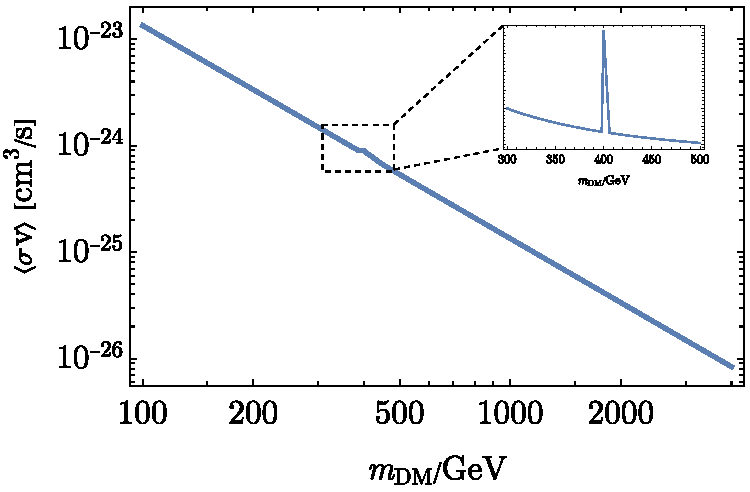
\includegraphics[height=1.8in]{Results/svCOMBINED.pdf}
%  \label{fig:test1}
\end{minipage}%
\centering
\begin{minipage}{.6\textwidth}
  \centering
  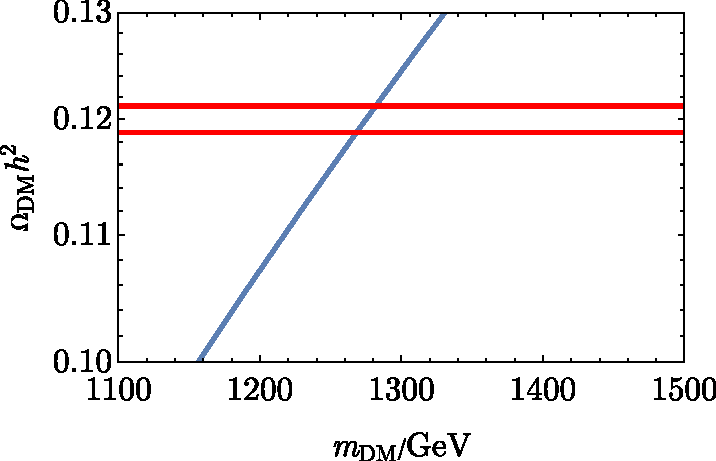
\includegraphics[height=1.9in]{Results/COMBINED.pdf}
%  \captionof{figure}{A figure}
%  \label{fig:test1}
\end{minipage}% 
\caption[\hspace{0.175in}Sección de choque térmica y densidad de materia oscura]{Sección de choque térmica y densidad de materia oscura considerando todos los canales de aniquilación de manera `democrática' ($g'=1$ en todos los casos).} 
\label{Results-COMBINED}
\end{figure}

\newpage

\section[\hspace{-0.14in}Conclusiones]{Conclusiones}
En este capítulo hemos estudiado al candidato a materia oscura $\mathcal{DM}$ dado por el escalar complejo $\mathcal{DM} = \eta_3^0$ con masa de orden $\mathcal{O}$(GeV$-$TeV). Para hacerlo estable, lo hicimos más ligero que los quarks pesados del $\nu_R-331$, prohibiendo su decaimiento por razones cinemáticas. 

Vimos que hay tres maneras en que este escalar puede aniquilarse y producir la abundancia de reliquia de las observaciones cosmológicas. Mostramos varios casos ilustrativos donde cada diagrama de Feynman es dominante (esto es, hacemos los demás acoples nulos) y verificamos que se puede hallar $\Omega_\mathcal{DM}h^2$ en el intervalo $[0.1188,0.1212]$.

También trabajamos el caso más general cuando todos los diagramas contribuyen `democráticamente' (todos los acoples iguales a 1) y hallamos la correcta abundancia de reliquia.
